%%%%%%%%%%%%%%%%%%%%%%%%%%%%%%%%%%%%%%%%%%%%%%%%%%%%%%%%%%%%%%%%%%%%%%
% Lớp 12 | Ứng dụng đạo hàm để khảo sát hàm số | Khảo sát sự biến thiên và vẽ đồ thị hàm số
% Dạng 2D1?5-3: Biện luận số giao điểm dựa vào đồ thị, bảng biến thiên
% Số câu: 9  (sinh tự động bởi tach_cau.py; từ nay thầy sửa trực tiếp file này)
%%%%%%%%%%%%%%%%%%%%%%%%%%%%%%%%%%%%%%%%%%%%%%%%%%%%%%%%%%%%%%%%%%%%%%

%%%%%%%%%%%%%%%% TRẮC NGHIỆM 4 PHƯƠNG ÁN %%%%%%%%%%%%%%%%

% nguồn: Phan1_Lop_12_Dai_so_Chuong_1
\begin{ex}%[2D1N5-3]%[ma:331a56c6]
		Cho hàm số  $y=f(x)$ có bảng biến thiên như sau:
		\begin{center}
			
\begin{tikzpicture}
				 \tkzTabInit[nocadre,espcl=2.5,lgt=1.5]
					{$x$/0.7,$f'(x)$/0.7,$f (x)$/2.1} 
					 {$-\infty$,$1$,$3$,$+\infty$}
				 \tkzTabLine{,-,0,+,0,-,}
				 \tkzTabVar{+/$+\infty$,-/$-1$,+/$3$,-/$-\infty$}
			\end{tikzpicture}
		\end{center}
		 Số nghiệm của phương trình $3f(x)+1=0$ là
	\choice 
			{$0$} 
			 {$1$}
			 {$2$}
			 {\True $3$}
	 \loigiai{
			Ta  có $3f(x)+1=0$ $\Leftrightarrow $ $f(x)=\dfrac{-1}{3}$.\\
		Vì đường thẳng $y=\dfrac{-1}{3}$ cắt đồ thị hàm  số $y=f(x)$ tại ba điểm phân biệt nên phương trình $3f(x)+1=0$ có ba nghiệm phân biệt.}
	\end{ex}

% nguồn: Phan1_Lop_12_Dai_so_Chuong_1
\begin{ex}%[2D1N5-3]%[ma:4580e08b]
		Cho hàm số $y=f(x)$  có bảng biến thiên như sau
		\begin{center}
			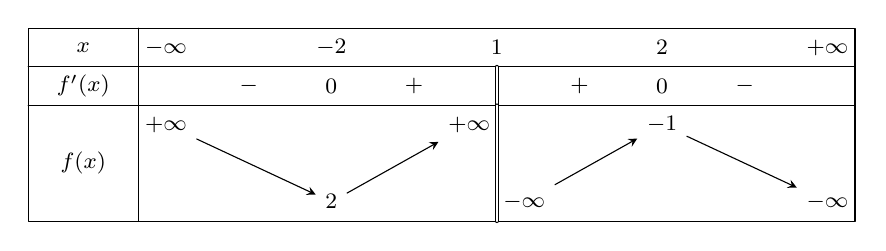
\begin{tikzpicture}[scale=.7,line join=round,line cap=round,font=\footnotesize,>=stealth]
				 \def\myltespcl{3}\def\myltlgt{2}\def\myltdeltacl{0.5}
				\def\myltx{0.7}\def\mylta{0.7}\def\myltb{2.1}\def\myltc{\myltb/3} 
				\path (\myltlgt/2,-\myltx/2) node  {$x$}
					(\myltlgt/2,-\myltx-\mylta/2)  node {$f'(x)$}
					(\myltlgt/2,-\myltx-\mylta-\myltb/2) node {$f  (x)$};
				\draw  (0,-\myltx)--(\myltlgt+4*\myltespcl+2*\myltdeltacl,-\myltx)
					(0,-\myltx-\mylta)--(\myltlgt+4*\myltespcl+2*\myltdeltacl,-\myltx-\mylta) 
					 (\myltlgt,0)--(\myltlgt,-\myltx-\mylta-\myltb);
				 \draw (0,0) rectangle (\myltlgt+4*\myltespcl+2*\myltdeltacl,-\myltx-\mylta-\myltb);
				\path (\myltlgt+\myltdeltacl,-\myltx/2) node  {$-\infty$};
				 \path (\myltlgt+\myltdeltacl+0.5*\myltespcl,-\myltx-\mylta/2) node {$-$};
				\path (\myltlgt+\myltdeltacl+\myltespcl,-\myltx/2) node  {$-2$};
				\path (\myltlgt+\myltdeltacl+1.5*\myltespcl,-\myltx-\mylta/2) node  {$+$};
				\path (\myltlgt+\myltdeltacl+2*\myltespcl,-\myltx/2)  node {$1$};
				 \draw[double](\myltlgt+\myltdeltacl+2*\myltespcl,-\myltx)--(\myltlgt+\myltdeltacl+2*\myltespcl,-\myltx-\mylta);
				\path (\myltlgt+\myltdeltacl+2.5*\myltespcl,-\myltx-\mylta/2) node {$+$}; 
				\path (\myltlgt+\myltdeltacl+3*\myltespcl,-\myltx/2) node {$2$}; 
				\path  (\myltlgt+\myltdeltacl+3.5*\myltespcl,-\myltx-\mylta/2) node {$-$};
				\path (\myltlgt+\myltdeltacl+4*\myltespcl,-\myltx/2)  node {$+\infty$};
				\path (\myltlgt+\myltdeltacl+\myltespcl,-\myltx-\mylta/2) node  {$0$};
				\path (\myltlgt+\myltdeltacl+3*\myltespcl,-\myltx-\mylta/2) node  {$0$};
				\node (nmylta) at (\myltlgt+\myltdeltacl,-\myltx-\mylta-0.5*\myltc)  {$+\infty$};
				\node (nmyltb)  at (\myltlgt+\myltdeltacl+\myltespcl,-\myltx-\mylta-2.5*\myltc) {$2$};
				 \draw[double](\myltlgt+\myltdeltacl+2*\myltespcl,-\myltx-\mylta) -- (\myltlgt+\myltdeltacl+2*\myltespcl,-\myltx-\mylta-\myltb);
				 \node (nmyltcl) at (\myltlgt+2*\myltespcl,-\myltx-\mylta-0.5*\myltc) {$+\infty$};
				 \node (nmyltcr) at (\myltlgt+2*\myltdeltacl+2*\myltespcl,-\myltx-\mylta-\myltb+0.5*\myltc) {$-\infty$};
				\node (nmyltd)  at (\myltlgt+\myltdeltacl+3*\myltespcl,-\myltx-\mylta-0.5*\myltc) {$-1$};
				\node (nmylte) at (\myltlgt+\myltdeltacl+4*\myltespcl,-\myltx-\mylta-2.5*\myltc)  {$-\infty$};
				 \draw[->] (nmylta)--(nmyltb);
				\draw[->]  (nmyltb)--(nmyltcl);
				\draw[->] (nmyltcr)--(nmyltd); 
				\draw[->] (nmyltd)--(nmylte); 
			\end{tikzpicture}
		\end{center}
		Số  nghiệm của phương trình $2f(x)-3=0$ là
	\choice 
			{\True  $0$}
			{$1$} 
			 {$2$}
			{$3$} 
	\loigiai{ 
			Đồ thị hàm số $y=f(x)$ không có điểm chung với đường thẳng $y=\dfrac{3}{2}$ nên  phương trình $f(x)=\dfrac{3}{2}$ hay $2f(x)-3=0$ vô nghiệm.
		} 
	\end{ex}

% nguồn: Phan1_Lop_12_Dai_so_Chuong_1
\begin{ex}%[2D1H5-3]%[ma:659df2b9]
	Cho hàm số bậc ba $y=f(x)$ có đồ thị là đường cong trong hình bên. Số nghiệm  thực của phương trình $f(x)=-1$ là
	\begin{center}
		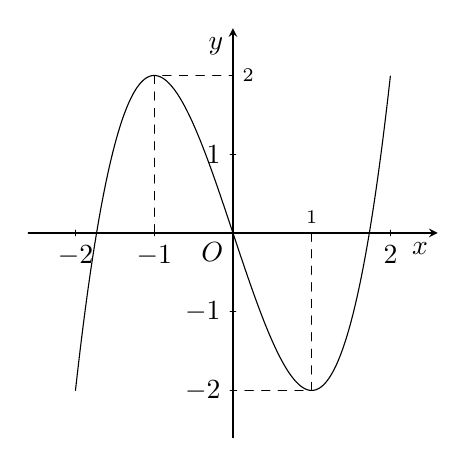
\begin{tikzpicture}[line join=round,line cap=round,>=stealth]
			 \tikzset{ethicknode/.style={scale=0.9}}
			 \draw[->] (-2.6,0)--(2.6,0) node[below left] {$x$};
			\draw[->] (0,-2.6)--(0,2.6) node[below  left] {$y$};
			 \draw (0,0) node [below left] {$O$};
			\foreach \x/\nx in {-2/-2,-1/-1,2/2} 
			\draw[thin] (\x,1pt)--(\x,-1pt)  node [below] {$\nx$};
			\node[above] at (1,0){\scriptsize  $1$};
			 \foreach \y/\ny in {-2/-2,-1/-1,1/1}
			\draw[thin] (1pt,\y)--(-1pt,\y)  node [left] {$\ny$};
			\node[right] at (0,2){\scriptsize  $2$};
			\draw[dashed,thin](-1,0)--(-1,2)--(0,2); 
			 \draw[dashed,thin](1,0)--(1,-2)--(0,-2);
			\begin{scope}
				\clip (-2.5,-2.5)  rectangle (2.5,2.5);
				\draw[samples=200,domain=-2:2,smooth,variable=\x] plot (\x,{1*((\x)^3)+0*((\x)^2)+-3*(\x)+0}); 
			\end{scope}
		\end{tikzpicture}
	\end{center}
	 \choice
		{\True  $3$}
		 {$1$}
		 {$0$}
		 {$2$}
	 \loigiai{
		Số nghiệm thực của  phương trình $f(x)=-1$ chính là số giao điểm của đồ thị hàm số $y=f(x)$ và đường thẳng $y=-1$.
		\begin{center}
			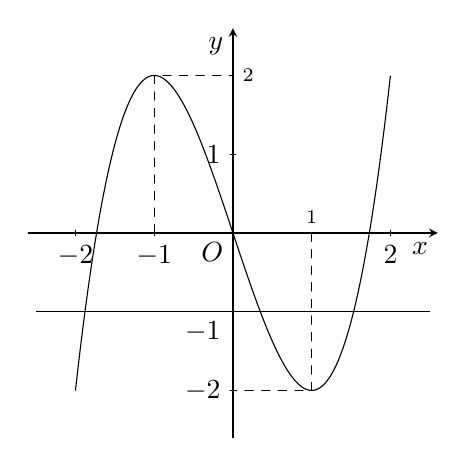
\begin{tikzpicture}[line join=round,line cap=round,>=stealth]
				 \tikzset{ethicknode/.style={scale=0.9}}
				\draw[->] (-2.6,0)--(2.6,0) node[below  left] {$x$};
				\draw[->] (0,-2.6)--(0,2.6)  node[below left] {$y$};
				 \draw (0,0) node [below left] {$O$};
				\foreach \x/\nx  in {-2/-2,-1/-1,2/2}
				\draw[thin]  (\x,1pt)--(\x,-1pt) node [below] {$\nx$};
				\node[above] at  (1,0){\scriptsize $1$};
				\foreach  \y/\ny in {-2/-2,1/1}
				\draw[thin] (1pt,\y)--(-1pt,\y)  node [left] {$\ny$};
				\node[right] at (0,2){\scriptsize  $2$};
				\foreach \z/\nz in {-1/-1} 
				\draw[thin] (1pt,\z)--(-1pt,\z) node [below  left] {$\nz$};
				\draw[dashed,thin](-1,0)--(-1,2)--(0,2); 
				\draw[dashed,thin](1,0)--(1,-2)--(0,-2); 
				\begin{scope}
					\clip (-2.5,-2.5)  rectangle (2.5,2.5);
					\draw[samples=200,domain=-2:2,smooth,variable=\x]  plot (\x,{1*((\x)^3)+0*((\x)^2)+-3*(\x)+0});
					\draw[samples=200,domain=-2.6:2.6,smooth,variable=\x]  plot (\x,{-1});
				\end{scope}
			\end{tikzpicture}
		\end{center}
		Từ hình vẽ suy ra phương  trình $f(x)=-1$ có $3$ nghiệm.
	} 
\end{ex}

% nguồn: Phan1_Lop_12_Dai_so_Chuong_1
\begin{ex}%[2D1V5-3]%[ma:cbe39364]
		Tìm tất cả các giá trị thực của tham số $m$ để đồ  thị hàm số $y=x^3-3x^2$ cắt đường thẳng $y=m$ tại ba điểm phân biệt.
	\choice 
			{$m\in  (-\infty;-4)$}
			{\True  $m\in (-4;0)$}
			 {$m\in (0;+\infty)$}
			{$m\in (-\infty;-4)\cup (0;+\infty)$} 
	 \loigiai{
			Ta có $y=x^3-3x^2 \Rightarrow y'=3x^2-6x;~y'=0 \Leftrightarrow \hoac{& x=0 \\& x=2.}$\\ 
			 Bảng biến thiên\\
			\begin{center}
				
\begin{tikzpicture}
					\tkzTabInit[espcl=2.5,lgt=1.5] 
						{$x$/0.7,$y'$/0.7,$y$/2.1} 
						{$-\infty$,$0$,$2$,$+\infty$} 
					\tkzTabLine{,+,0,-,0,+,} 
					\tkzTabVar{-/$-\infty$,+/$0$,-/$-4$,+/$+\infty$} 
				\end{tikzpicture}
			\end{center}
			 Dựa vào bảng biến thiên ta thấy đồ thị hàm số $y=x^3-3x^2$ cắt đường thẳng $y=m$ tại ba điểm phân biệt khi $-4<m<0$.
		} 
	\end{ex}


%%%%%%%%%%%%%%%% ĐÚNG/SAI %%%%%%%%%%%%%%%%

% nguồn: Phan1_Lop_12_Dai_so_Chuong_1
\begin{ex}%[2D1N5-3]%[ma:825e415b]
	Cho hàm  số $y=\dfrac{x^2-x-1}{x-2}$ có đồ thị là $(C)$.
	\choiceTF 
		{Đồ thị hàm số có một  tiệm cận ngang}
		{\True Đồ thị hàm số cắt trục tung tại điểm $M$. Phương trình tiếp tuyến của đồ thị hàm số tại $M$ là $3x-4y+2=0$} 
		{Đồ thị $(C)$ có hai điểm cực trị nằm 2 phía  đối với $Oy$}
		{Đồ  thị không cắt trục $Ox$}
	 \loigiai{
		Tập xác  định $\mathbb{D}=\mathbb{R}\setminus\{2\}$.\\
		Ta  có đạo hàm $y'=\dfrac{x^2-4x+3}{(x-2)^2}$ và $y'=0\Leftrightarrow\heva{&x=1\\&x=3.}$\\
		Bảng biến  thiên
		\begin{center}
\begin{tikzpicture}[>=stealth]
		\tkzTabInit[nocadre=false,lgt=1,espcl=2,deltacl=0.5]{$x$/.7,$y'$/.7,$y$/2} 
			 {$-\infty$,$1$,$2$,$3$,$+\infty$}
		 \tkzTabLine{,+,$0$,-,d,-,$0$,+,}
		 \tkzTabVar{-/$-\infty$,+/$1$,-D+/$-\infty$/$+\infty$,-/$5$,+/$+\infty$}
	\end{tikzpicture}
		\end{center}
		\begin{itemchoice}
			 \itemch Ta có $\lim\limits_{x\to+\infty}y=+\infty$, $\lim\limits_{x\to-\infty}y=-\infty$ nên đồ thị hàm số không có tiệm cận ngang.
			\itemch Giao điểm của đồ thị hàm số với trục tung là $M\left(0;\dfrac{1}{2}\right)$ và $y'(0)=\dfrac{3}{4}$  nên phương trình tiếp tuyến của đồ thị hàm số tại $M$ là $y=\dfrac{3}{4}x+\dfrac{1}{2}$.
			\itemch Hàm  số đạt cực trị tại $x=1$ và $x=3$ nên 2 điểm cực trị nằm cùng phía đối với $Oy$.
			\itemch Ta có $y=\dfrac{x^2-x-1}{x-2}=0\Leftrightarrow\begin{cases}x=\dfrac{1-\sqrt{5}}{2}\\x=\dfrac{1+\sqrt{5}}{2}
		\end{cases}$ Do đó giao điểm của đồ thị hàm số với trục hoành là $\left(\dfrac{1-\sqrt{5}}{2}; 0\right)$ và $\left(\dfrac{1+\sqrt{5}}{2}; 0\right)$.
	\end{itemchoice}
} 
\end{ex}

% nguồn: Phan1_Lop_12_Dai_so_Chuong_1
\begin{ex}%[2D1V5-3]%[ma:570ac284]
	Cho hàm số $y=\dfrac{x^2+3x+3}{x+2}$  có đồ thị là đường cong $(C)$
	\choiceTF 
		{Biết hàm số có hai điểm cực trị khi đó tổng của giá trị cực  đại và giá trị cực tiểu bằng $-4$}
		{\True Đường tiệm cận xiên  của đồ thị hàm số đi qua điểm $A(0;1)$}
		{\True Phương trình tiếp tuyến  với $(C)$ vuông góc với đường thẳng $x-3y-6=0$ đi qua điểm $B\left(-\dfrac{3}{2};\dfrac{3}{2}\right)$}
		{Để phương trình $x^2+3x+3=m|x+2|$ có 4 nghiệm  phân biệt thì $m>2$}
	\loigiai{ 
		\begin{itemchoice}
			\itemch  $y'=\dfrac{x^2+4x+3}{(x+2)^2}=0\Leftrightarrow\hoac{&x=-1\Rightarrow y=1\\&x=-3\Rightarrow y=-3.}$
			 Bảng biến thiên:
			\begin{center}
\begin{tikzpicture}[>=stealth]
		 \tkzTabInit[nocadre=false,lgt=1,espcl=2,deltacl=0.5]{$x$/.7,$y'$/.7,$y$/2}
			 {$-\infty$,$-1$,$1$,$-3$,$+\infty$}
		\tkzTabLine{,-,$0$,+,d,+,$0$,-,} 
		\tkzTabVar{+/$+\infty$,-/$1$,+D-/$+\infty$/$-\infty$,+/$-3$,-/$-\infty$} 
	\end{tikzpicture}
			\end{center}
			Dựa vào bảng biến thiên ta có $y_{\text{ CĐ}}+y_{\text{ CT}}=-2$. 
			\itemch $\lim\limits_{x\to-2^\pm}y=\pm\infty$: $x=-2$ là tiệm cận đứng;\\ $\lim\limits_{x\to\pm\infty}y-(x+1)=0\Rightarrow y=x+1$ là tiệm cận xiên.\\ 
			Do  đó tiệm cận xiên của đồ thị hàm số đi qua $A(0;1)$.
			\itemch Đường thẳng $x-3y-6=0$ có hệ số  góc $k_1=\dfrac{1}{3}\Rightarrow$ tiếp tuyến của $(C)$ vuông góc với đường thẳng này có hệ số góc $k_2=-3$.\\
			Xét phương trình\\ $y'=-3\Leftrightarrow\dfrac{x^2+4x+3}{(x+2)^2}=-3\Leftrightarrow\begin{cases}x\ne-2\\x^2+4x+3=-3x^2-12x-12
		\end{cases}$
		$\Leftrightarrow\begin{cases}x\ne-2\\4x^2+16x+15=0
	\end{cases}\Leftrightarrow \hoac{&x=-\dfrac{5}{2}\Rightarrow y=-\dfrac{7}{2}.\\&x=-\dfrac{3}{2}\Rightarrow y=\dfrac{3}{2}.}$
	Tại $A\left(-\dfrac{5}{2};-\dfrac{7}{2}\right)$ có tiếp tuyến $(T_1): y=-3\left(x+\dfrac{5}{2}\right)-\dfrac{7}{2}\Leftrightarrow y=-3x-11$. 
	Tại $B\left(-\dfrac{3}{2};\dfrac{3}{2}\right)$  có tiếp tuyến $(T_2): y=-3\left(x+\dfrac{3}{2}\right)+\dfrac{3}{2}\Leftrightarrow y=-3x-3$.
	\itemch Xét phương trình $x^2+3x+3=m|x+2|\Leftrightarrow\begin{cases}x\ne-2\\\dfrac{x^2+3x+3}{|x+2|}=m
	\end{cases}\Rightarrow$
	Xét hàm số $y=\dfrac{x^2+3x+3}{|x+2|}=\begin{cases}\dfrac{x^2+3x+3}{x+2}&(1): x>-2\\-\dfrac{x^2+3x+3}{x+2}&(2): x<-2
	\end{cases}$\\
	(1): Đồ thị của (1) là phần đồ thị  $(C)$ nằm bên phải đường tiệm cận đứng.\\
	(2): Đồ thị của (2) là phần đối xứng với phần đồ thị $(C)$ ở bên trái đường tiệm cận đứng qua trục $Ox$.\\ 
	Số giao điểm của  $(C_1)$ và đường thẳng $y=m$ là số nghiệm của phương trình.\\
	Vị  trí của đường thẳng $y=m$ để có 4 giao điểm với $(C_1)$ là $m>3$.
	\end{itemchoice}
} 
\end{ex}


%%%%%%%%%%%%%%%% TRẢ LỜI NGẮN %%%%%%%%%%%%%%%%

% nguồn: Phan2_Lop_12_Dai_so_Chuong_1
\begin{bt}%[2D1H5-3]%[ma:39fa8ca9]
	\immini{Cho hàm số $f(x)$  liên tục trên $\mathbb{R}$ và có đồ thị của hàm $y=f'(x)$ như hình vẽ. Phương trình $f(x)=f(3)$ có bao nhiêu nghiệm?}
	{	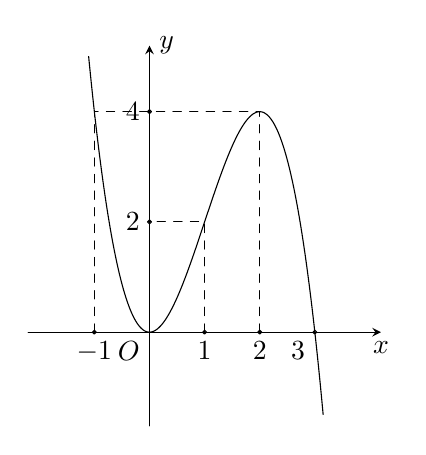
\begin{tikzpicture}[scale=0.7,line join=round,line cap=round,>=stealth]
		 \tikzset{ethicknode/.style={scale=1}}
		\def\xmin{-2}\def\xmax{4}\def\ymin{-1.5}\def\ymax{5} 
		\draw[->] (\xmin-0.2,0)--(\xmax+0.2,0) node[below]{$x$}; 
		 \draw[->] (0,\ymin-0.2)--(0,\ymax+0.2) node[right]{$y$};
		\draw (0,0) node[below  left]{$O$};
		\foreach \x  in {-1,1,2}\draw (\x,0)--(\x,0) circle (1pt) node[below]{$\x$};
		\foreach  \y in {2,4}\draw (0,\y)--(0,\y) circle (1pt) node[left]{$\y$};
		 \clip (\xmin,\ymin) rectangle (\xmax,\ymax);
		 \draw[smooth,samples=200,domain=-1.5:3.5] plot (\x,{-1*((\x)^3)+3*((\x)^2)});
		\draw (3,0)  circle (1pt) node[below left]{$3$};
		\draw[dashed] (-1,0) --  (-1,4) -- (0,4);
		\draw[dashed] (1,0)  -- (1,2) -- (0,2);
		\draw[dashed] (2,0)  -- (2,4) -- (0,4);
	\end{tikzpicture}
	 }
	\shortans{1} 
	 \loigiai{
		Từ đồ thị của hàm số $y=f'(x)$, ta suy ra dạng bảng biến thiên của  hàm $y=f(x)$ như sau
		\begin{center}
			
\begin{tikzpicture}
				\tkzTabInit[nocadre=true,lgt=1.2,espcl=2.5,deltacl=0.6] 
					{$x$ /0.6,$y’$ /0.6,$y$  /2}
					{$-\infty$,$0$,$3$,$+\infty$} 
				\tkzTabLine{,+,0,+,0,-,} 
				\tkzTabVar{-/,R/,+/$f  (3)$,-/}
			\end{tikzpicture}
		\end{center}
		Từ đây, ta suy ra  số nghiệm của phương trình $f(x)=f(3)$ là $1$ nghiệm.
	 }
\end{bt}

% nguồn: Phan2_Lop_12_Dai_so_Chuong_1
\begin{bt}%[2D1V5-3]%[ma:2414c6bd]
	Tất cả các giá trị của tham số $m$ sao cho đồ thị hàm số  $y = x^3 - 3x^2 + 3m - 1$ cắt trục hoành tại ba điểm phân biệt trong đó có đúng hai điểm có hoành độ lớn hơn $1$ là khoảng $(a;b)$. Giá trị của $a + 3b$ bằng bao nhiêu?
	 \shortans{6}
	\loigiai{ 
		Ta có: $y' = 3x^2 - 6x;\ y' = 0 \Leftrightarrow 3x^2 -  6x = 0 \Leftrightarrow \hoac{&x = 0\\&x = 2.}$\\
		Bảng biến thiên 
		\begin{center}
			\begin{tikzpicture}
				\tkzTabInit[nocadre=false,lgt=1.5,espcl=3,deltacl=0.5] 
					{$x$/1,$f’(x)$/1,$f  (x)$/4}
					 {$-\infty$,$0$,$1$,$2$,$+\infty$}
				\tkzTabLine{,-,z,,,+,,,} 
				\draw 
					 (N13) node[above](A){$-\infty$}
					(N22)  node[below](B){$3m-1$}
					 ($(N22)!0.5!(N43)$) node (C){$3m-3$}
					(N43)  node[above](D){$3m-5$}
					(N52) node[below](E){$+\infty$}; 
				\draw[-stealth] (A)--(B); 
				\draw[-stealth] (B)--(C); 
				\draw[-stealth]  (C)--(D);
				\draw[-stealth] (D)--(E); 
			\end{tikzpicture}
		\end{center}
		Từ bảng biến thiên ta thấy: Đồ thị hàm số cắt trục hoành  tại ba điểm phân biệt trong đó có đúng hai điểm có hoành độ lớn hơn $1$ khi và chỉ khi:
		\[ 
		3m - 5 < 0  < 3m - 3 \Leftrightarrow (3m - 3)(3m - 5) < 0 \Leftrightarrow 1 < m < \dfrac{5}{3}.
		\] 
		 Từ đó suy ra $a = 1$, $b = \dfrac{5}{3}$ nên $a + 3b = 6$.
	} 
\end{bt}


%%%%%%%%%%%%%%%% TỰ LUẬN %%%%%%%%%%%%%%%%

% nguồn: Phan2_Lop_12_Dai_so_Chuong_1
\begin{bt}%[2D1C5-3]%[ma:93d75649]
	Cho hàm  số $y=f(x)$ liên tục trên $\left[1;3 \right]$ và có bảng biến thiên như sau
	\begin{center}
		
\begin{tikzpicture}
			 \tkzTabInit[espcl=2.5,lgt=1.5]
				{$x$/0.7,$f'(x)$/0.7,$f  (x)$/2.1}
				 {$1$,$2$,$3$}
			 \tkzTabLine{,+,0,-,}
			 \tkzTabVar{-/$1$,+/$4$,-/$3$}
		\end{tikzpicture}
	\end{center}
	Có bao nhiêu giá trị nguyên của  $m$ để phương trình $f\left( x+1 \right)=\dfrac{m}{x^{2}-4x+5}$ có nghiệm trên khoảng $\left( 1;2 \right)$?
	 \loigiai{
		Vì  $x^{2}-4x+5=\left( x-2 \right)^{2}+1>0, \forall x\in \mathbb{R}$ nên $f\left( x+1 \right)=\dfrac{m}{x^{2}-4x+5}\Leftrightarrow \left( x^{2}-4x+5 \right)f\left( x+1 \right)=m$.\\
		Đặt $h\left( x \right)=\left( x^{2}-4x+5 \right)f\left( x+1 \right)$ với  $x\in \left( 1;2 \right)$. \\
		Ta có  $h'\left( x \right)=\left( x^{2}-4x+5 \right)f'\left( x+1 \right)+\left( 2x-4 \right)f\left( x+1 \right)$. \\
		Dựa vào bảng biến thiên của hàm số $y=f\left( x \right)$, ta có $\forall x\in \left( 1;2 \right)\Rightarrow x+1\in \left( 2;3 \right)\Rightarrow f'\left( x+1 \right)\leqslant 0$  và $2x-4<0,\forall x\in \left( 1;2 \right);f\left( x+1 \right)\geqslant 3>0,x+1\in \left( 2;3 \right)$. \\
		Do đó, $h'\left( x \right)<0,\forall x\in  \left( 1;2 \right)$. \\
		Bảng biến  thiên của hàm số $h\left( x \right)$ trên khoảng $\left( 1;2 \right)$ như sau
		\begin{center}
			
\begin{tikzpicture}
				\tkzTabInit[espcl=2.5,lgt=1.5] 
					{$x$/0.7,$h'(x)$/0.7,$h  (x)$/2.1}
					{$1$,$2$} 
				 \tkzTabLine{,-,}
				\tkzTabVar{+/$h (1)$,-/$h (2)$} 
			\end{tikzpicture}
		\end{center}
		Khi đó, phương trình $h\left( x \right)=m$ có nghiệm $x\in \left( 1;2  \right)$ khi và chỉ khi $h\left( 2 \right)<m<h\left( 1 \right)$ \\
		$\Rightarrow 1\cdot f\left( 3  \right)<m<2.f\left( 2 \right)\Leftrightarrow 3<m<8$. \\
		Vì $m$ nguyên nên  $m\in\{4;5;6;7\}$.\\
		Vậy  có $4$ giá trị nguyên của $m$ thỏa mãn yêu cầu bài toán.
	} 
\end{bt}
